\documentclass[10pt,letterpaper]{article} 
%\usepackage{tikz}
%\usepackage{tools}
\usepackage{amsmath,amssymb,geometry,graphicx,enumitem,caption,subcaption}
%\usefonttheme{serif}‎
%\usepackage{ptext}‎
%\usepackage{xepersian}
%\settextfont{B Nazanin}
\usepackage{lipsum}
\setlength{\parindent}{0pt}
\newcommand{\pf}{$\blacksquare$}
\newcommand{\Q}[1]{\textbf{Question #1)}}
\newcommand{\EX}{\Bbb E}
\newcommand{\nl}{\newline\newline}
\providecommand{\pic}[2]{
\begin{center}
\includegraphics[width=#2]{#1}
\end{center}
}
\begin{document}
\Large
\begin{center}
In the name of beauty

The 1st problem set of Optical Networks course

\hrulefill
\end{center}
\Q1

\begin{enumerate}[label=\alph*)]
\item
Explain what WDM stands for in terminology and what it means in adequate words. How do WDM systems enhance optical transmission versus the classical, non-WDM systems?
\item
Why are EDFAs needed in an optical system? Where are they typically placed in a network architecture?
\item
Compare the backbone and access networks from responsibility, economical consideration and number of wavelengths per fiber points of view.
\item
Mention the major differences between OTN and SONET/SDH protocols by their provided bit rates and framing.
\item
Which of the broadcast-and-select, route-and-select and wavelength-selective architectures are contentionless? Which one support multicast? Elaborate your response.
\end{enumerate}

\Q2

In the following 4-node network, the circle-shaped, triangle-shaped and interleaved ovals denote nodes, EDFAs and spools of fiber respectively.
\begin{figure}[ht]
\centering
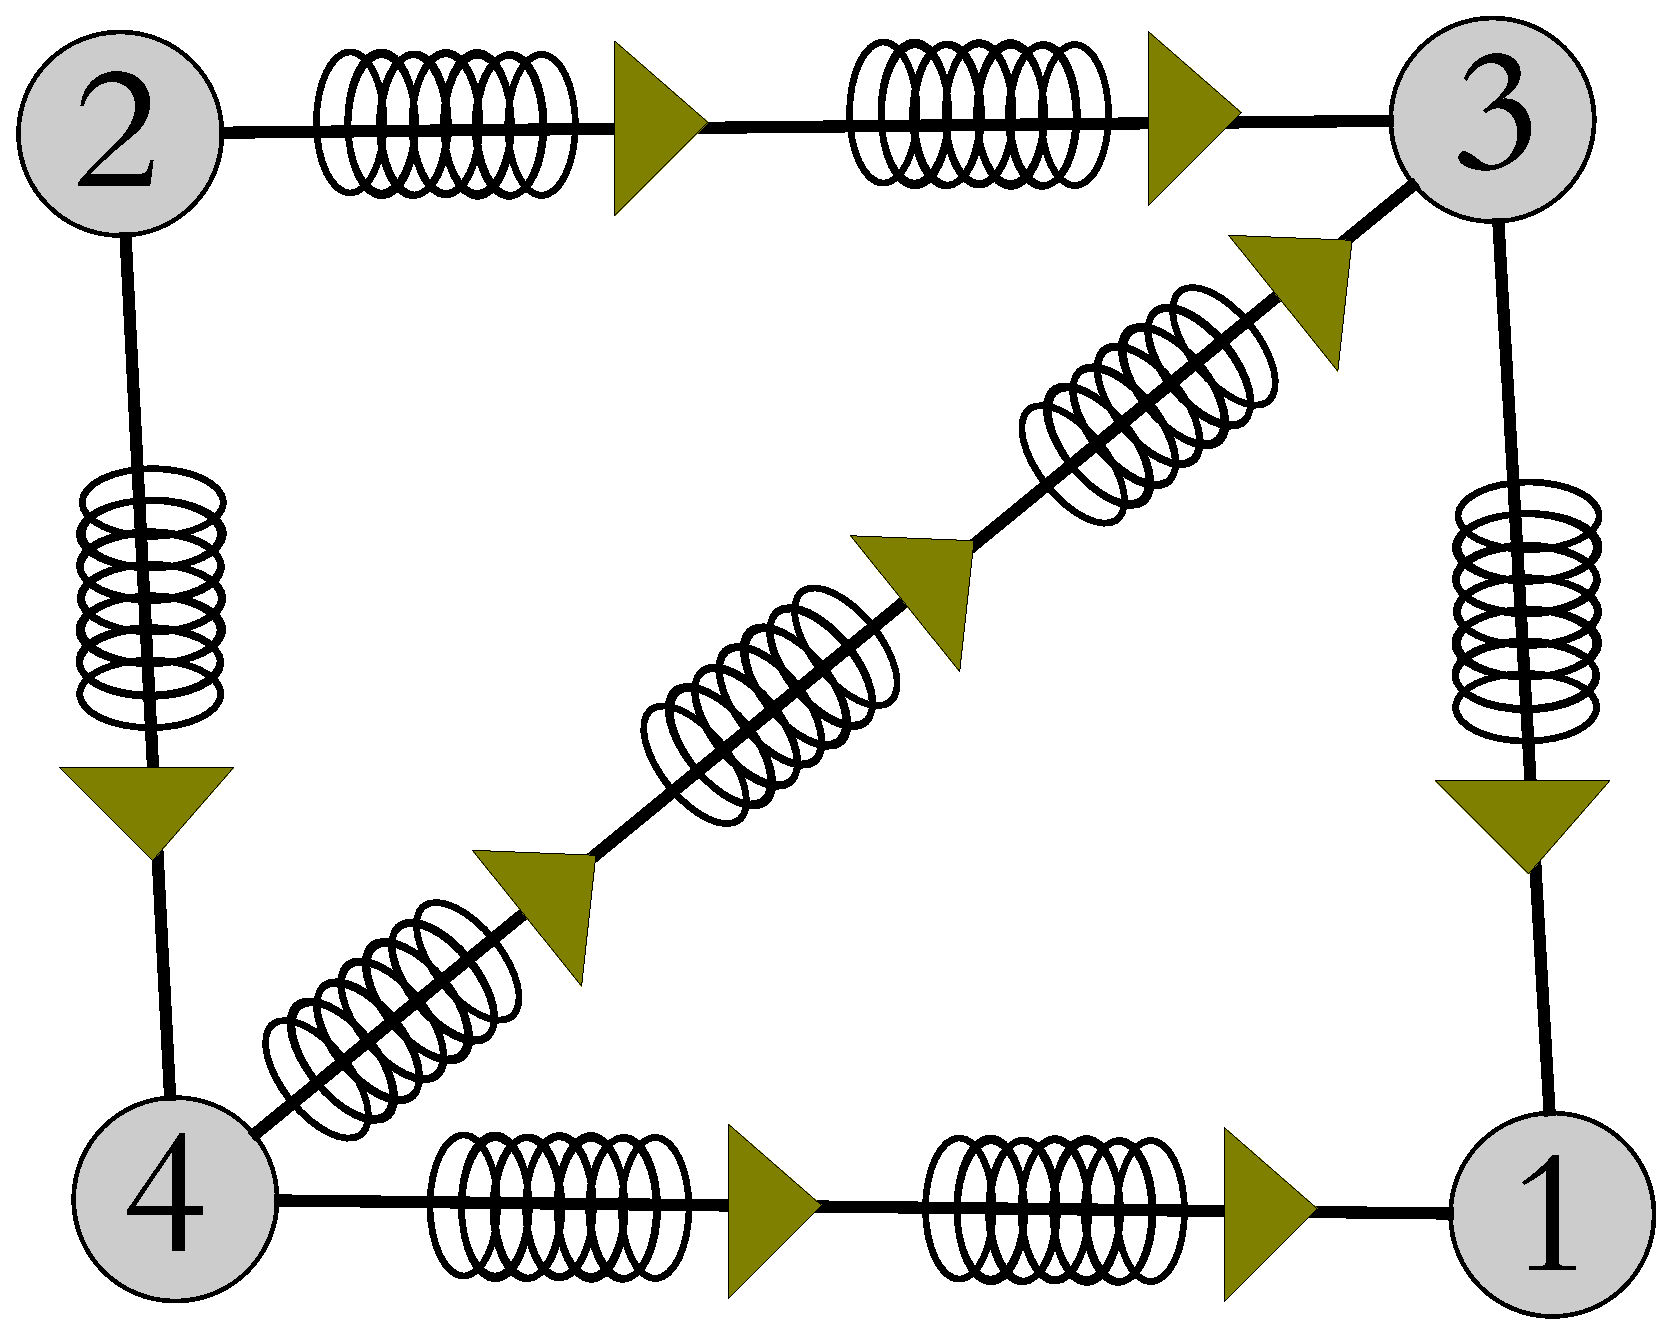
\includegraphics[scale=0.3]{PS1_Net}
\end{figure}
\begin{enumerate}[label=\alph*)]
\item
What is the formal definition of link and how many links are in the network?
\item
What is the formal definition of span and how many spans are in the network?
\item
List the degrees of the nodes in order of their labels.
\item
Typically inside a node architecture, there are amplifiers called \textit{pre-amplifier} on each input link entering and boosters on each output link exiting from the node. Mention two nodes with maximum number of boosters and pre-amplifiers distinctly.
\end{enumerate}

%a. Which of the four tiers in an optical network (backbone [which is also called core or long-haul], regional, metro-core and access) are more cost-sensitive and what do you think about the reason?
%
%b. Mention some different technology implementations in tiers of an optical network and enrich your answer with enough explanations.
%
%c. What are the pros and cons of \textit{protocol and format transparency}?

\Q3

\begin{enumerate}[label=\alph*)]
\item
Why is the problem of Network Engineering treated as semi-static compared with Traffic Engineering which is considered as dynamic?
\item
Is conversion between client-side and network-side signals performed \textit{all optically}? Why or why not?
\item
Based on the difference between grooming and multiplexing, which one gives rise to more efficiency and why?
\item
What are the advantages and shortcomings of using Wavelength-Selective Switch (WSS) in place of Array Wave-guide Grating (AWG)?
\end{enumerate}

\Q4

Consider the following $3\times 5$ grid network where every link is 1,000 km in length. Assume that all nodes support optical bypass and that the optical reach is 3,000 km. Assume that there is one wavelength of traffic in both directions between every pair of nodes. What is the average nodal drop ratio in this network, assuming all connections are routed over the shortest distance path? The average nodal drop ratio is defined as
$$
\frac
{\sum_i\text{Number of Wavelengths that Drop At Node $i$}}
{\sum_i\text{Number of Wavelengths that Enter Node $i$}}
$$
\begin{figure}[ht]
\centering
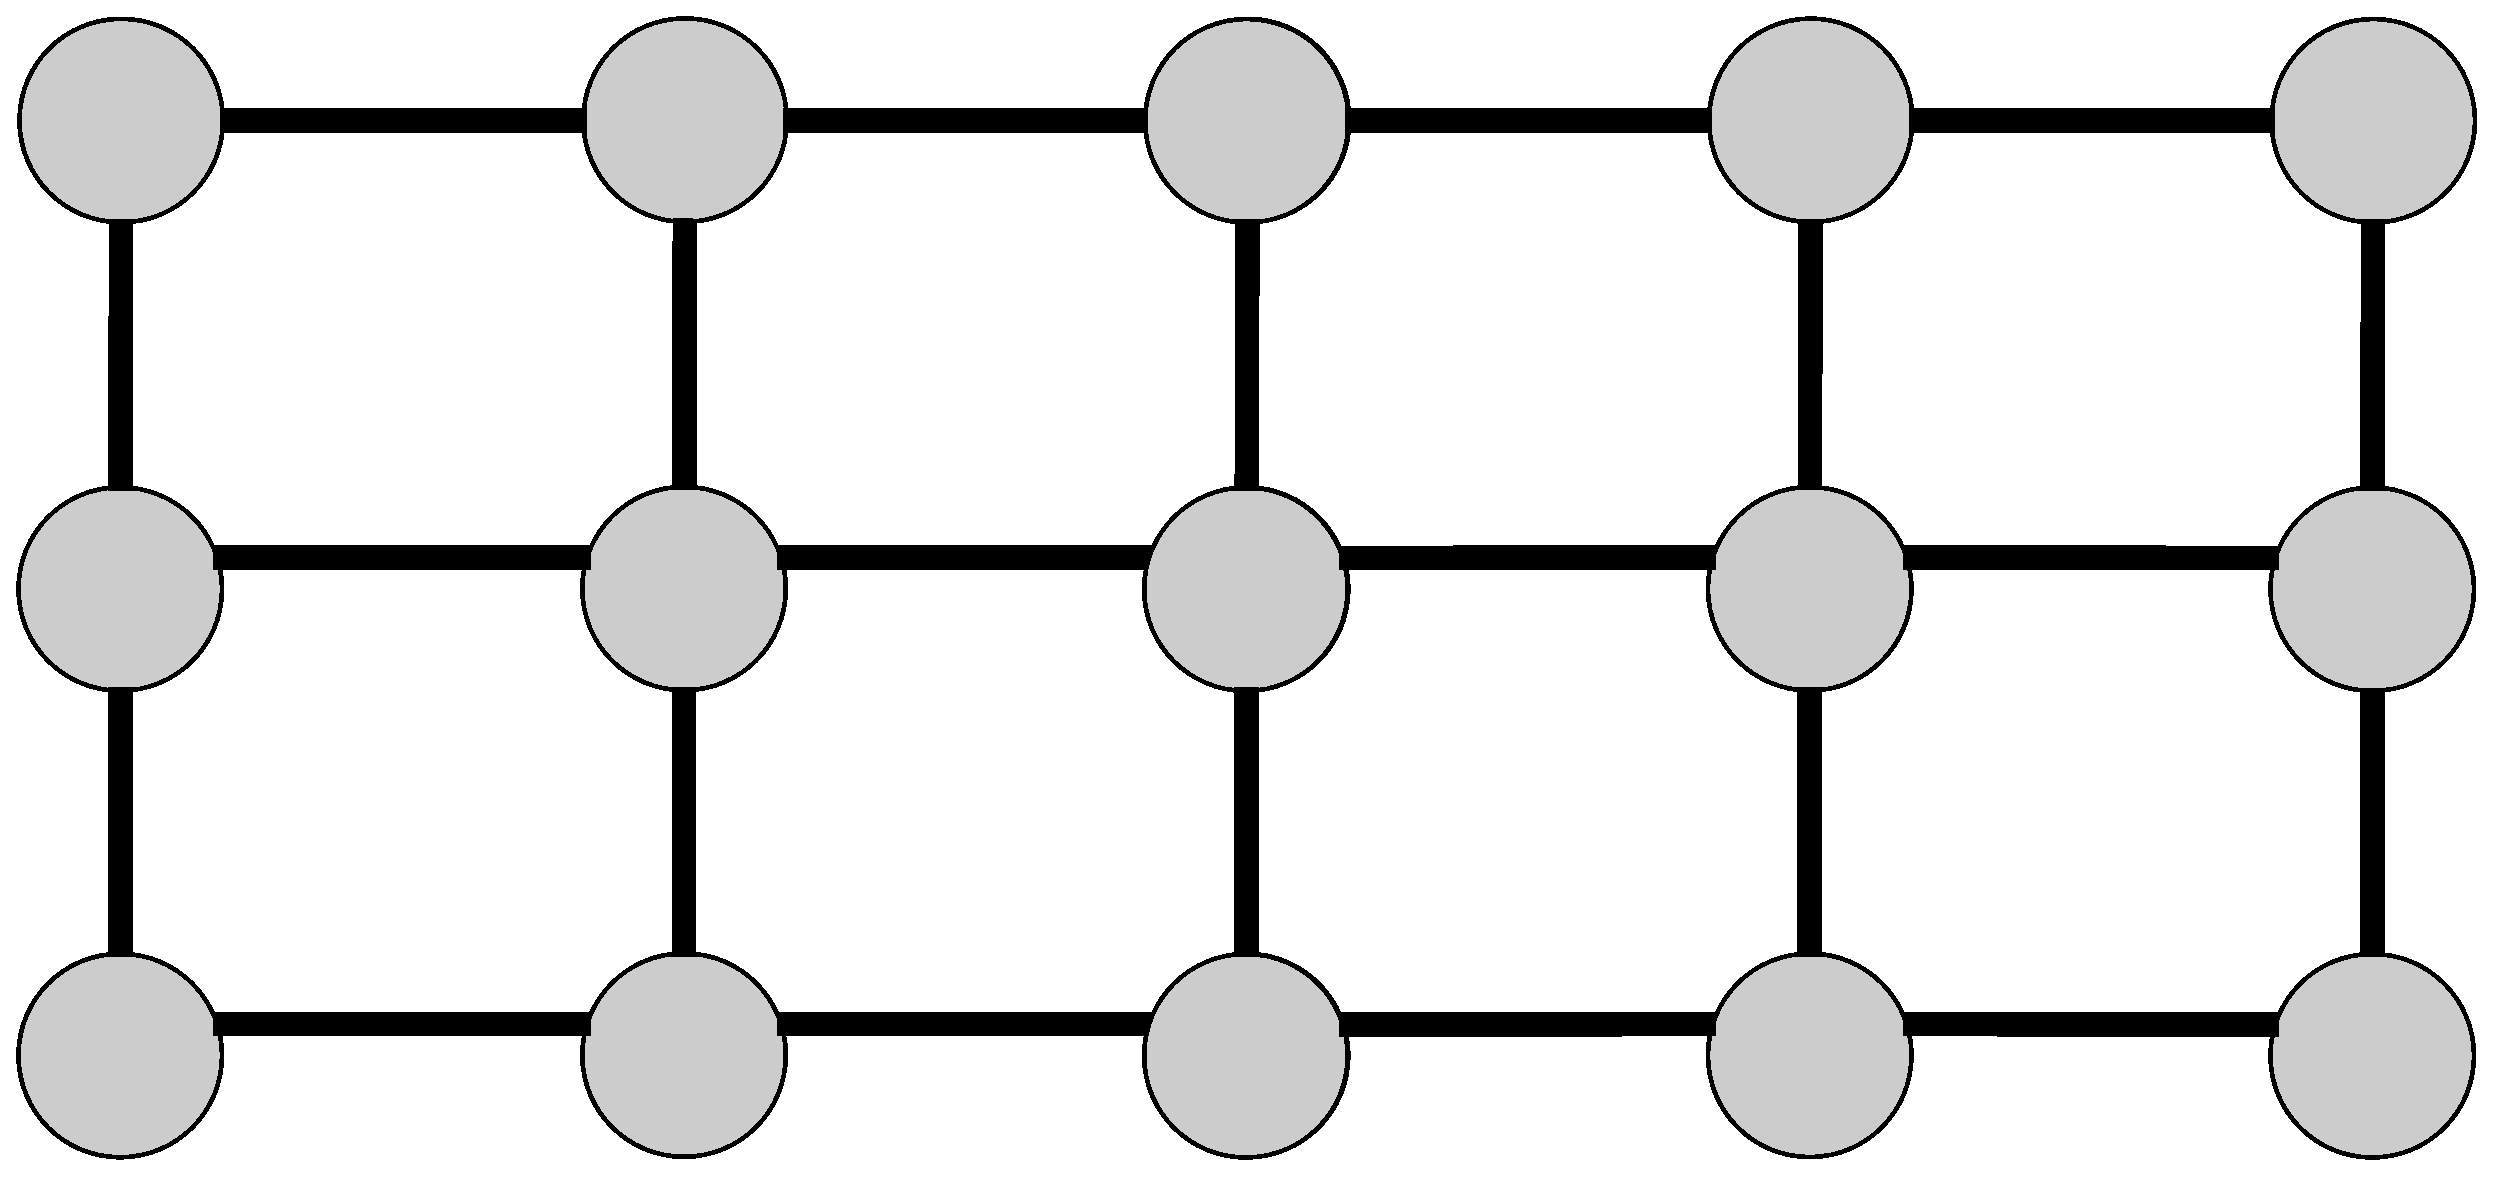
\includegraphics[scale=0.2]{PS1_Simmons}
\end{figure}

\Q5

Consider constructing an $M\times N$ WSS by cascading one $M\times$ WSS with one $1\times N$ WSS.
\begin{enumerate}[label=\alph*)]
\item
Is this $M\times N$ WSS internally contentionless?
\item
If the answer to part (a) is negative, can a contentionless $M\times N$ WSS be constructed from multiple $M\times 1$ WSSs and multiple
$1\times N$ WSSs?
\item
If you answered part (b) affirmatively, how many of these WSSs are needed?
\end{enumerate}
(Note: For cost reasons, the $M\times N$ WSS is ideally constructed as an integrated component; the designs explored here are for investigating the functionality.)

\Q6

Consider the following optical-terminal architecture, with one passive splitter and multiple $1\times N$ WSSs. An alternative architecture can be constructed with one $1\times N$ WSS followed by multiple passive splitters. For example, if $4N$ transponders need to be supported on the terminal, the $1\times N$ WSS directs 4 wavelengths to each output port, and the passive splitters are of size $1\times 4$. Compare this architecture to that of the question figure, on criteria such as high-level cost, loss, multicasting capability, etc.
\begin{figure}[ht]
\centering
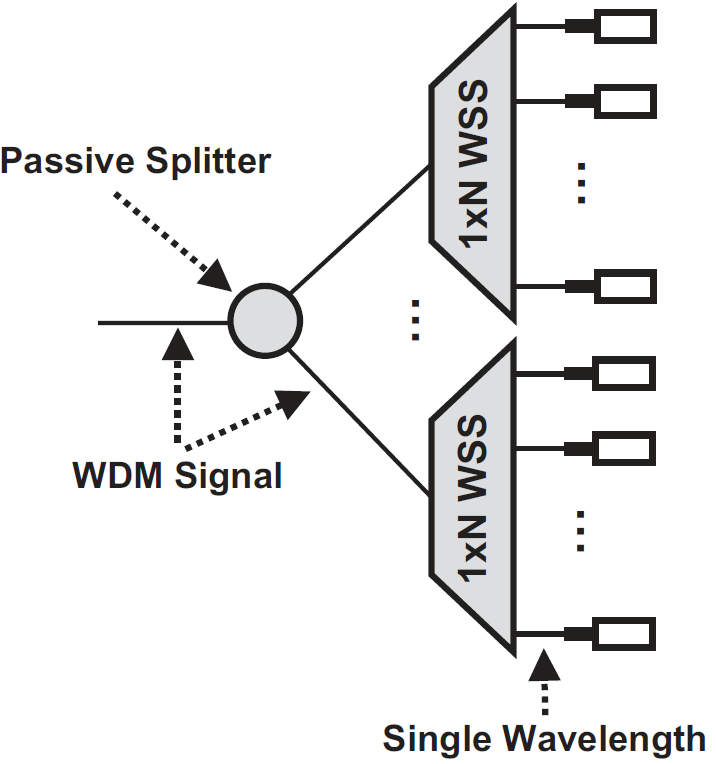
\includegraphics[scale=0.3]{PS1_OET}
\end{figure}

\Q7

Consider a degree-$N$ node with $W$ wavelengths per fiber, where up to a fraction $P$ of the total wavelengths at the node may add/drop. Consider a core switch at the node that operates on all incoming/outgoing wavelengths and all add/drop wavelengths, and an edge switch that operates only on the add/drop wavelengths, both of which illustrated in the next page. Both switches are assumed to have a per-wavelength granularity.
\begin{enumerate}[label=\alph*)]
\item
What is the general formula for how large of a core switch is required at this node?
\item
What is the general formula for how large of an edge switch is required at this node?
\item
What is the ratio of the two switch sizes?
\end{enumerate}
\begin{figure}[ht]
\centering
%%%%%%%%%%%%%%%%%%%
\begin{subfigure}{0.49\textwidth}
\centering
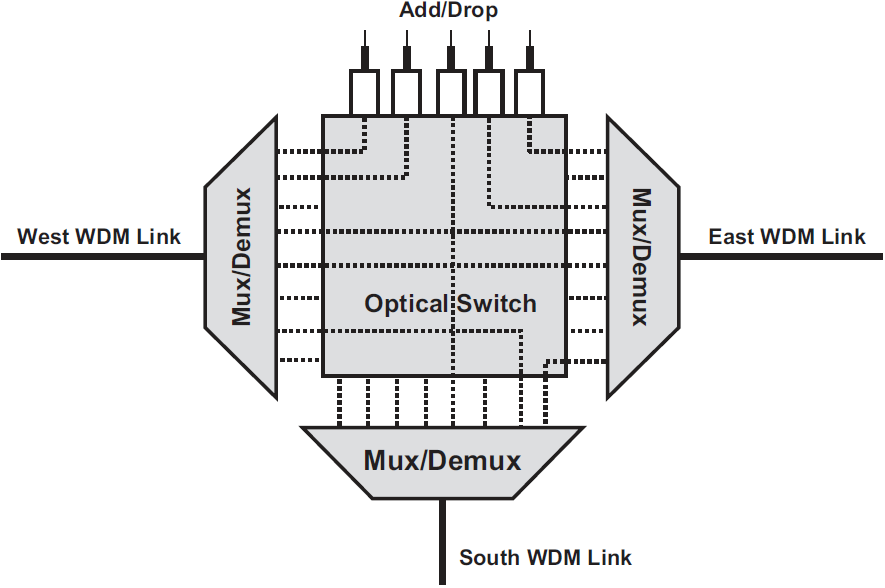
\includegraphics[scale=0.35]{Core_Switch}
\caption{Core Switch}
\end{subfigure}
%%%%%%%%%%%%%%%%%%%
\begin{subfigure}{0.49\textwidth}
\centering
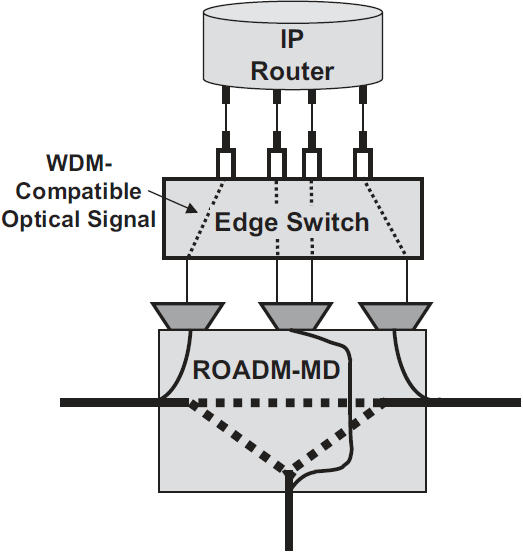
\includegraphics[scale=0.4]{Edge_Switch}
\caption{Edge Switch}
\end{subfigure}
%%%%%%%%%%%%%%%%%%%
\end{figure}
%\nl
%\Q5 
\end{document}